% !TeX root = ../Book2.tex
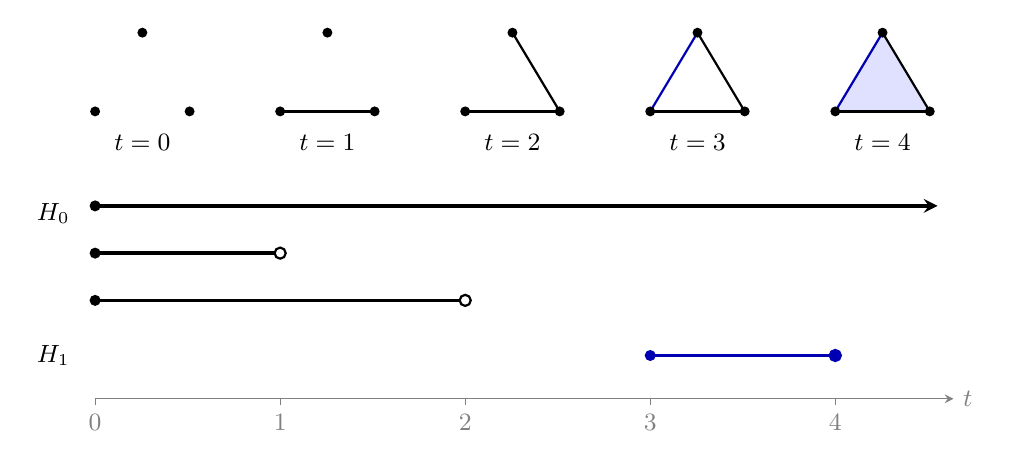
\begin{tikzpicture}[>=stealth,every node/.style={font=\small},x=1cm,y=1cm]
	\foreach \k in {0,1,2,3,4} {
		\begin{scope}[xshift={2.35*\k cm}]
			\ifnum\k=4 \fill[blue!12] (0,0)--(1.2,0)--(.6,1)--cycle;\fi
			\ifnum\k>0 \draw[thick] (0,0)--(1.2,0);\fi
			\ifnum\k>1 \draw[thick] (1.2,0)--(.6,1);\fi
			\ifnum\k>2 \draw[thick,blue!70!black] (.6,1)--(0,0);\fi
			\foreach \p in {(0,0),(1.2,0),(.6,1)} \fill \p circle (1.8pt);
			\node at (.6,-.4) {\(t=\k\)};
		\end{scope}
	}
	\node[left] at (-.2,-1.3) {\(H_0\)};
	\node[left] at (-.2,-3.1) {\(H_1\)};
	\draw[gray,->] (0,-3.65)--(10.9,-3.65) node[right] {\(t\)};
	\foreach \k in {0,1,2,3,4} {
		\draw[gray] ({2.35*\k},-3.65)--({2.35*\k},-3.73) node[below] {\(\k\)};
	}
	\draw[very thick,->] (0,-1.2)--(10.7,-1.2);
	\fill (0,-1.2) circle (2pt);
	\draw[very thick] (0,-1.8)--(2.35,-1.8);
	\fill (0,-1.8) circle (2pt);
	\draw[fill=white,thick] (2.35,-1.8) circle (2pt);
	\draw[very thick] (0,-2.4)--(4.7,-2.4);
	\fill (0,-2.4) circle (2pt);
	\draw[fill=white,thick] (4.7,-2.4) circle (2pt);
	\draw[very thick,blue!70!black] (7.05,-3.1)--(9.4,-3.1);
	\fill[blue!70!black] (7.05,-3.1) circle (2pt);
	\draw[fill=white,thick,blue!70!black] (9.4,-3.1) circle (2pt);
\end{tikzpicture}
